\chapter{Ogólny opis rozwiązania}
\label{cha:opis}

\section{Cel projektu}
\label{sec:celProjektu}

Celem projektu jest stworzenie aplikacji internetowej dodającej do tradycyjnych map dodatkowego wymiaru, czasu. Powinna dostarczać możliwości obserwowania zmian zachodzących na określonym terenie w danym okresie. Dodana oś czasu będzie miała za zadanie kontrolowanie okresu dla którego widoczne będą dane. Dostarczone dane przez użytkownika będą przedstawiane jemu w czytelny i umożliwiający szybką analizę sposób. Przykładowe dane wejściowe to zmiany terytorialne w przeszłości, ukazanie rozowuju miast. Końcowa wizualizacja danych oprócz prostych kształtów geometrycznych musi zapewniać obsłógę zewnętrznych plików graficznych jak i najnowszych rozwiązań służących do obsługi grafiki.

\section{Problemy do rozwiązania}
\label{sec:problemy}

\begin{itemize}

\item
Przechowywanie i transmisja danych

Nie jest określony jeden format danych który będzie używany w aplikacji. Oprócz informacji opisujących położenie punktów zawarte również będą szczegółowe dane dotyczące ich wyglądu i zachowania, również obrazy graficzne mogą się znajdować w opisie mapy.

\item
Wizualizacja

Szeroki zakres informacji który może opisywać mapę musi być odpowiednio wyświetlany, w sposób czytelny i ułatwiający analizę dużych zbiorów danych. W jednym miejscu zostaną zebrane różnego rodzaju dane które muszą współpracować ze sobą tworząc spójną kompozycję.

\item
Bezpieczeństwo

Dane dostarczane przez zewnętrzny serwer powinny być wiarygodne. Użytkonwik posiadający kopię pliku znajdującą się na dysku lokalnym z infromacjami o mapię musi mieć możwliwość sprawdzenia jej autentyczności z aktualną wersją na serwerze.

\item
Optymalizacja rozwiązania

Aplikacja musi w każdym momencie zapewniać płynną pracę. Praca  ze szczegółową mapą posiadającą wiele informacji musi przebiegać płynnie, bez dużych opóźnień.

\end{itemize}

\section{Użytkownicy}
\label{sec:uzytkownicy}

\begin{itemize}
\item
Administrator

Osoba która posiada dostęp do serwera na krórym działa aplikacja korzystająca z omawianego frameworku. Ponieważ tworzony program jest jedynie narzędziem służącym do pracy z interaktywnymi mapami, a jednym z założeń jest jak największa adaptabliność i mozliwość działania na różnych środowiskach wymagana jest osoba która doda do działającej strony aplikację.
\item
Moderator

Pzygotowanie i edycja map powinna być wykonana przez uprawnione osoby. Może to być na przykład osoba posiadającą dużą wiedzę na dany temat, posiada ona możliwość edycji mapy.
\item
Uczeń

Użytkownik z najmniejszymy uprawnieniami, jedynie do przeglądania mapy.
\end{itemize}

\section{Granice systemu}
\label{sec:granicesystemu}

System umożliwia moderatorowi:
\begin{itemize}
\item
Tworzenie i edycję zestawów danych przechowywanych na serwerze

\item 
Tworzenie własnych filtrów edytujących mapę w zależności od jej położenia lub czasu

\item
Zapis informacji o mapie do pliku na dysku lokalnym

\end{itemize}

System umożliwia uczniowi:
\begin{itemize}
\item
Przeglądanie gotowych map

\item
Pracę bez konieczności stałego dostępu do internetu.

\item
Sprawdzanie autentyczności pliku przy pomocy obliczania sumy kontrolnej

\end{itemize}

System nie umożliwia:
\begin{itemize}
\item
Wykorzystywania plików video

\end{itemize}

\section{Lista możliwości}
\label{sec:listamozliwosci}

Praca z mapami w trybie offline
\begin{itemize}
\item
Wczytywanie pliku - dane używane w aplikacji mogą zostać wczytane z dwóch źródeł. Z lokalnego dysku lub zaimportowane z serwera.

\item
Przechywanie danych po stornie klienta 

\end{itemize}

Szeroki wachlarz dostęnych sposobów wizualizacji danych
\begin{itemize}
\item
Korzystanie z grafiki wektorowej

\item
Współpraca z plikami graficznymi

\item
Obsługa animacji poprzez svg

\end{itemize}

Współpraca z zewętrznymi aplikacjami
\begin{itemize}
\item
Obłsuga plików GML

\item
Parsowanie danych z formatu xml to pamięci storage

\end{itemize}

Tworzenie interaktywnych filtów
\begin{itemize}
\item
Filtry obsługjące zminę czasu

\item
Filtry obsługujące zmianę mapy

\end{itemize}

test

\section{Specyfikacja wymagań}
\label{sec:specyfikacja wymagan}

\subsection{Ogólny diagram przypadków użycia}
\label{sec:diagramcaseuse}


\begin{center}
\begin{figure}[H]
\centering
     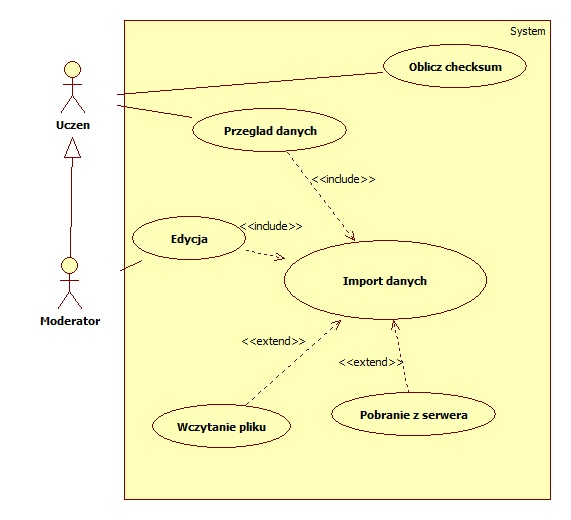
\includegraphics[origin=c,width=130mm]{ge/caseuse.jpg}
      \caption{Case use.}
       \label{fig:caseuse}
\end{figure}
\end{center}

\subsection{Definicje przypadków użycia}
\label{sec:defCaseuse}

Poniżej znajduje się opis trzech podstawowych przypadków użycia występujących w aplikacji. Opisane zostały warunki rozpoczęcia każdego z nich i ich zakończenia, zarówno pozytywnego jak i negatywnego.

\begin{table}[H]
    \centering
    \begin{tabular}{|l<{\raggedright}|p{3in}|}
    \hline
    Nazwa przypadku uzycia & Wczytanie danych z pliku  \\ \hline
    Typ przypadku uzycia  & Ogólny  \\ \hline
    Aktorzy   & Uczeń    \\ \hline
    Warunki wstepne   & Brak     \\ \hline
    Warunku koncowe dla sukcesu   & Dane zostaja zapisane w pamieci lokalnej przegladarki    \\ \hline
    Warunki koncowe dla niepowodzenia   & Dane nie sa poprawnie odczytane.     \\ \hline
    Scenariusz glówny   &

    \begin{enumerate}
    \itemsep0em
        \item Uzytkownik wybiera plik.
        \item Dane podlegaja parsowaniu.
        \item Poprawnie odczytane dane zostaja zapisane w Storage.
    \end{enumerate}
     \\ \hline
    Scenariusz alternatywny   &

    \begin{enumerate}
    \itemsep0em
        \item Uzytkownik wybiera plik.
        \item Dane podlegaja parsowaniu.
        \item Dane nie zostaja odczytane poprawnie.
        \item Uzytkownik zostaje poinformowany o zainstnialym bledzie.
    \end{enumerate}
         \\ \hline
    \end{tabular}
    \caption{Przypadek wczytania danych}
    \label{tab:caseuse1}
\end{table}

\begin{table}[H]
    \centering
    \begin{tabular}{|l<{\raggedright}|p{3in}|}
    \hline
    Nazwa przypadku użycia & Wyświetlenie danych \\ \hline
    Typ przypadku użycia  & Ogólny  \\ \hline
    Aktorzy   & Uczeń     \\ \hline
    Warunki wstępne   & Dane znajdują się w pamięci lokalnej     \\ \hline
    Warunku końcowe dla sukcesu   & Dane zostają wyświetlone     \\ \hline
    Warunki końcowe dla niepowodzenia   & Mapa nie jest aktualizowana     \\ \hline
   Scenariusz glówny   &

    \begin{enumerate}
    \itemsep0em
        \item Uzytkownik wybiera punkt w czasie.
        \item Dane dla wybranego okresu zostają wyrenderowane i pokazane.
        \item Informacje dla najbliższego otoczenia podlegają generacji i ukryciu.
    \end{enumerate}
     \\ \hline
    Scenariusz alternatywny   &

    \begin{enumerate}
    \itemsep0em
        \item Uzytkownik wybiera punkt w czasie.
        \item Dane dla wybranego okresu nie zostają odnalezione
        \item Nie aktualne dane zostają schowane.
    \end{enumerate}
         \\ \hline
    \end{tabular}
    \caption{Przypadek wyświetlenia danych}
    \label{tab:caseuse2}
\end{table}

\begin{table}[H]
    \centering
    \begin{tabular}{|l<{\raggedright}|p{3in}|}
    \hline
    Nazwa przypadku użycia & Walidacja autentyczności pliku  \\ \hline
    Typ przypadku użycia  & Ogólny  \\ \hline
    Aktorzy   & Uczeń    \\ \hline
    Warunki wstępne   & Uczeń posiada plik na dysku i jego sumę kontrolną z serwera    \\ \hline
    Warunku końcowe dla sukcesu   & Pojawienie się komunikatu o autentyczności pliku    \\ \hline
    Warunki końcowe dla niepowodzenia   & Ostrzeżenie o dokonaniu zmian w pliku     \\ \hline
   Scenariusz glówny   &

    \begin{enumerate}
    \itemsep0em
        \item Uzytkownik wybiera zakładkę do walidacji pliku.
        \item Podanie ścieszki do pliku i sumy kontolnej.
        \item Obliczenie aktualnej sumy dla pliku i porównanie go z podanym.
        \item Uzytkownik zostaje poinformowany o poprawności pliku.
    \end{enumerate}
     \\ \hline
    Scenariusz alternatywny   &

    \begin{enumerate}
    \itemsep0em
        \item Uzytkownik wybiera zakładkę do walidacji pliku.
        \item Podanie ścieszki do pliku i sumy kontolnej.
        \item Obliczenie aktualnej sumy dla pliku i porównanie go z podanym.
        \item Uzytkownik zostaje poinformowany o zmianach w pliku.
    \end{enumerate}
         \\ \hline
    \end{tabular}
    \caption{Przypadek 2...}
    \label{tab:caseuse2}
\end{table}

\subsection{Wymagania niefunkcjonalne}
\label{sec:niefunkcjonalnes}

Oprócz wymagań dotyczących prawidłowego funkcjonowania aplikacji, wymagane jest
aby zapewnione były poniższe punkty.

\begin{itemize}
\item
The first item

\item
System powinien być skalowalny, powinien umożliwiać dostęp wielu użytkownikom równocześnie przy zachowaniu wymagań wydajnościowych.

\item
Aplikacja powinna działać identycznie na różnych środowiskach i przeglądarkach internetowych.
\end{itemize}
